\section{Introdu\c{c}\~ao}
\label{sec:introduction}
Fun\c{c}\~oes hash s\~ao amplamente utilizadas em v\'arias \'areas da
Ci\^encia da Computa\c{c}\~ao. 
Uma \textit{fun\c{c}\~ao hash} $h: U \to M$ mapeia chaves de um universo $U$, $|U|=u$, 
para um dado intervalo de inteiros $M=[0,m-1]=\{0,1,\dots,m-1\}$.
Seja~$S\subseteq U$ um subconjunto de $n$ chaves do universo $U$.
Dado uma chave~$k\in S$, uma fun\c{c}\~ao hash $h$ computa um inteiro em 
$M$ para armazenamento ou recupera\c{c}\~ao de $k$ em uma \textit{tabela hash}.
Neste artigo consideramos que as chaves s\~ao strings de bits de comprimento 
m\'aximo $L$. Portanto $u = 2^L$. 

M\'etodos de hashing para {\em conjuntos n\~ao est\'aticos} de chaves podem ser usados para
construir estruturas de dados para armazenar $S$ e suportar consultas do tipo
``$k \in S$?'' em tempo esperado $O(1)$.
No entanto, eles envolvem um certo desperd\'{\i}cio de espa\c{c}o e tempo devido
a localiza\c{c}\~oes inutilizadas na tabela e tempo para resolver colis\~oes quando duas
chaves s\~ao mapeadas para a mesma localiza\c{c}\~ao na tabela.


For {\em static sets} of keys it is possible to compute a function
to find any key in a table in one probe; such hash functions are called
\textit{perfect}. 
Given a set of keys~$S$, we shall say that a hash function~$h:U\to M$ is a
\textit{perfect hash function} for~$S$ if~$h$ is an injection on~$S$,
that is, there are no \textit{collisions} among the keys in~$S$: if~$x$
and~$y$ are in~$S$ and~$x\neq y$, then~$h(x)\neq h(y)$.
Figure~\ref{fig:minimalperfecthash-ph-mph}(a) illustrates a perfect hash
function.
Since no collisions occur, each key can be retrieved from the table
with a single probe.
If~$m=n$, that is, the table has the same size as~$S$,
then~$h$ is a \textit{minimal perfect hash function} for~$S$.
Figure~\ref{fig:minimalperfecthash-ph-mph}(b) illustrates
a~minimal perfect hash function.
Minimal perfect hash functions totally avoid the problem of wasted
space and time.

% For two-column wide figures use
\begin{figure}
% Use the relevant command to insert your figure file.
% For example, with the graphicx package use
\centering
  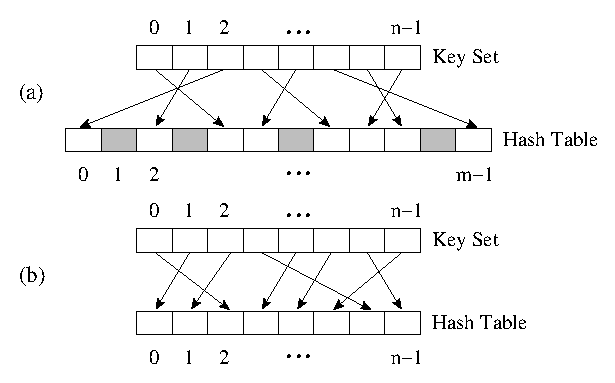
\includegraphics[width=0.45\textwidth, height=0.3\textheight]{figs/minimalperfecthash-ph-mph.ps}
% figure caption is below the figure
\caption{(a) Perfect hash function\quad  (b) Minimal perfect hash function}
\label{fig:minimalperfecthash-ph-mph}
\end{figure}

A efici\^encia dos algoritmos ser\'a medida atrav\'es das seguintes m\'etricas:
\begin{enumerate}
\item Quantidade de tempo gasto para encontrar uma fun\c{c}\~ao hash perfeita m\'{\i}nima $h$.
\item Quantidade de tempo necess\'ario para avaliar ou computar $h$.
\item Quantidade de mem\'oria exigida para armazenar a descri\c{c}\~ao da fun\c{c}\~ao $h$.
\item Quantidade de mem\'oria exigida para encontrar $h$.  
\item Escalabilidade dos algoritmos a medida que o conjunto de chaves cresce. 
\end{enumerate}

